%Directional part
\chapter{Analysis of Non-Directional Algorithm}
As our lower bound is based on directional algorithms, in this section, 
we will discuss whether there exists a non-directional algorithm 
which is faster than the lower bound.
Specifically, we claim that for the probability distribution defined in the previous section,
there is a deterministic directional algorithm whose expected cost is lower than or
equal to the expected cost of any deterministic non-directional algorithm.

\section{Definition}
Let $\sigma$ be a non-directional leaf ordering,
$\sigma'$ be the corresponding canonical ordering, and
$\sigma'_h$ be the subsequence of $\sigma$ containing only vertices
at height $h$ or lower.
Let $v$ be the first non-omitted vertex
at which $\sigma'$  differs from any directional algorithm.
Let $h$ be $v$'s height and let $t$ be $v$'s logical time-stamp.
Note that $t \geq 1$ since there is always a depth-first traversal
that starts from any leaf.
Let $u$ be the last vertex that precedes $v$ in $\sigma'$, and 
let $w$ be $u$'s parent.

\section{Analysis of three different cases of Non-Directional Algorithm}
The proof proceeds by analysing the three cases in which 
a non-directional algorithm can fall into.
\subsection{Non-Directional Algorithm Case 1}

In this case, $u$ and $v$ are siblings and $u$ is the last vertex that precedes $v$ in $\sigma'_h$. Vertex $w$'s value could be determined by vising $u$, non-directional algorithm 1 will go straight to visit $v$ but not omitting it.:
\begin{figure}[H]
	\centering
	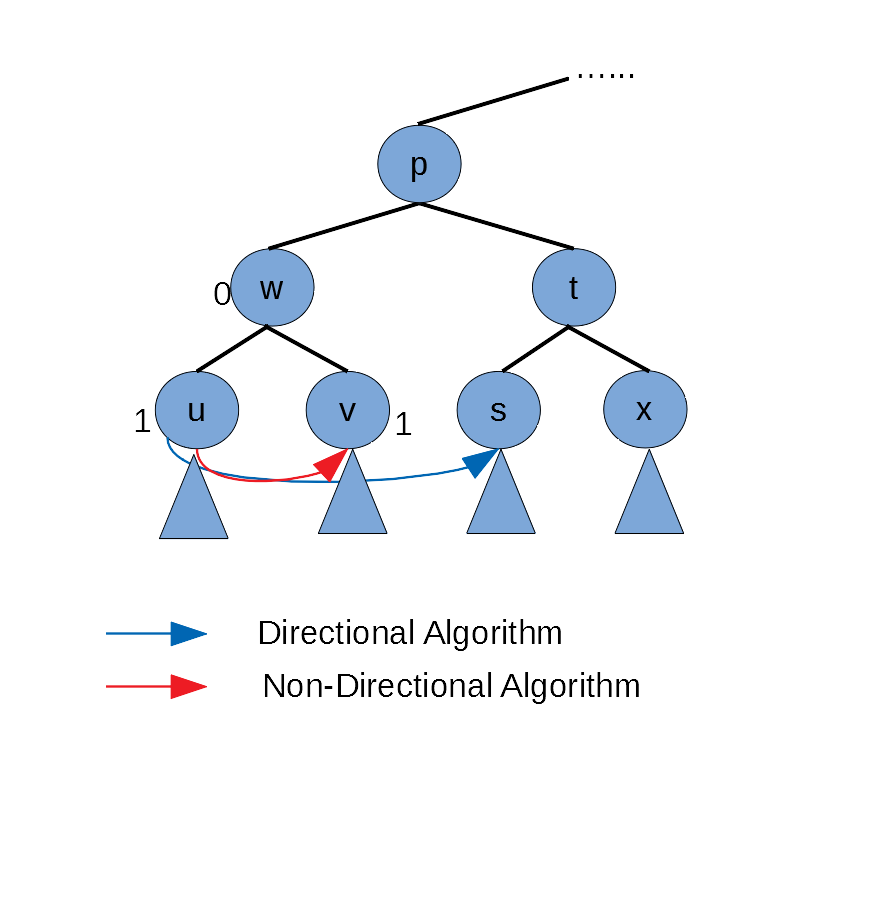
\includegraphics[width=0.7\linewidth]{nondir}
	\caption{ Non-Directional Algorithm case 1}
	\label{fig:nondir}
\end{figure}
\begin{proof}
	For case 1.If $u$ and $v$ are siblings, then the non-deterministic algorithm omits $v$ because it can determine the value of $w$ by visiting .Vertex $w$'s value could be determined only when $u$ is true and $w$ must be $false$. According to section 4, we already know that 
	this means $v$'s value could also been determined as false. Therefore, for any non-directional algorithm who evaluate $v$, the time for this process is wasted. 
	
	In conclusion, this case non-directional algorithm could not be faster than directional algorithm
\end{proof}

\subsection{Non-Directional Algorithm Case 2}
   In this case. $u$ and $v$ are not siblings, but their parents are siblings. Vertex $u$ could not determine the $w$'s value, but instead of visiting its sibling, non-directional algorithm 2 jumps out to visit $v$, who is in another sub tree. After visiting vertex $v$, there are two small cases: either jump back to visit $z$, or continue by visiting $y$. The non-directional algorithm 2 follows the figure below:
   \begin{figure}[H]
   	\centering
   	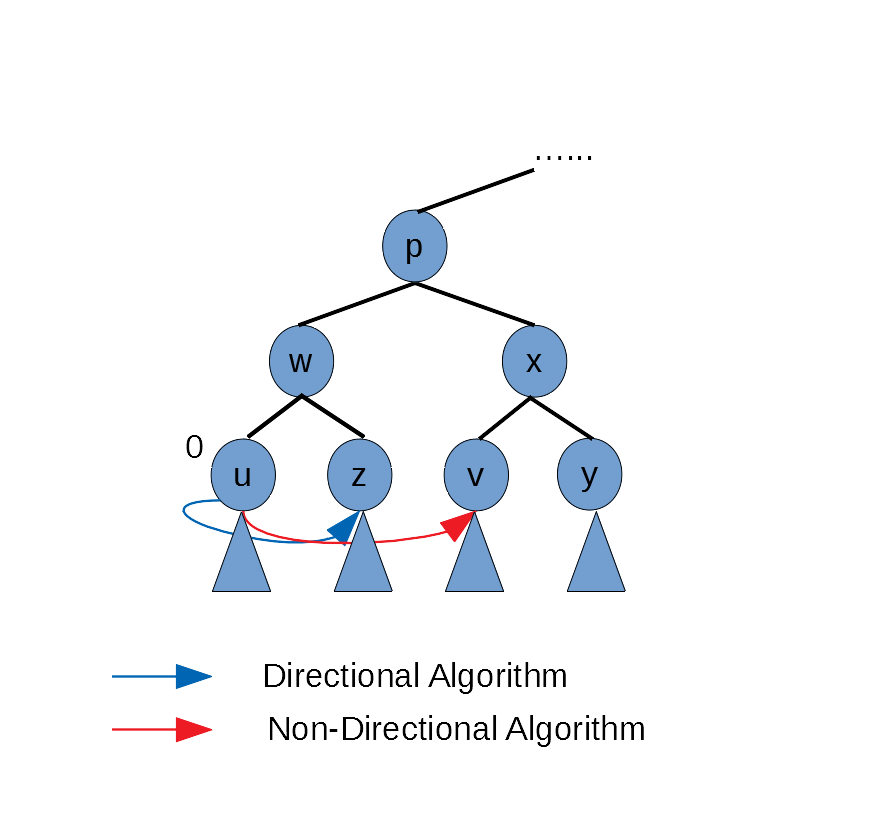
\includegraphics[width=0.7\linewidth]{nondir_case2}
   	\caption{Non-Directional Algorithm case 2}
   	\label{fig:nondircase2}
   \end{figure}

   If $u$ and $v$ are not siblings but at the same level, the non-directional algorithm 2 will visit $v$ when $w$'s value has not been determined. This non-directional algorithm will take advantage when only by visiting $v$ and its sibling could determine $p$'s value and z should be omitted. In this situation, $u$'s value should be 0, and $x$'s value should be 1. Therefore $v$ and its sibling $y$'s value should be 0, and $p$'s value should also be $0$.$z$ should be 1, because if $z$ is 0, then $p$'s value could be determined by directional algorithm by visiting $z$ after $u$, the visit of $u$ in non-directional algorithm is a waste. Let's prove it is also faster for trees of height n by induction. 
   
   Assumption: $E(c_N(x))$ depends only on the height of the tree rooted at $x$ and on the value of vertex $x$, but it does not depend on the state of the algorithm (for example, it is immaterial whether $x$ is the first or second child visited in the tree rooted at $x$'s parent). 
   
   E.g. $E(c_N(x)|w=1,x=0)$ actually does not include $E(c_N(u)|w=1,x=0)$, it just includes expectation of node $v$ and node $y$. This means though at this state of algorithm, of which we must evaluate vertex $u$ first before the evaluation process of vertex $x$, the expectation of evaluation cost of $x$ is not affected by the expectation of $u$. It should just determined by its own sub-trees' expectation. Otherwise we could say that, the expectation of a vertex is just determined by its own structure, but not by algorithm.
\begin{proof}       
   Assuming that directional algorithm is faster than or equal to non-directional algorithm for trees of height 1,2,...,n-1. For nor-tree of height n:
   Let $E(c(s))$ be the expected cost of an vertex $s$ in directional algorithm and $E(c_N(s))$ be the expected cost of an vertex $s$ in non-directional algorithm. Let $P,X,W$ be situation when $w=0,x=0$, $w=0,x=1$ and $w=1,x=0$
   The expected cost of directional algorithm is:
   \begin{equation}
   \begin{aligned}
   	E(c(p))=Pr[P]E[c(w)|P]+Pr[P]E[c(x)|P]+\\
   	Pr[X]E[c(w)|X]+Pr[X]E[c(x)|X]+Pr[W]E[c(w)|W]
   \end{aligned}
   \end{equation} 
   
   For the non-directional algorithm, there are two sub-cases. 
   If the algorithm continues to visit vertex $y$ before going back to $z$, then:
   \begin{equation}
   \begin{aligned}
     E(c_N(p))=Pr[P]E[c_N(w)|P]+Pr[P]E[c_N(x)|P]+Pr[X]E[c_N(u)|X]+\\
     Pr[X]E[c_N(x)|X]+Pr[W]E[c_N(w)|W]+Pr[W]E[c_N(x)|W]
   \end{aligned}
   \end{equation}
   	
   For jumping back to $z$'s case:
   \begin{equation}
   \begin{aligned}
   	E(c_N(p))=Pr[P]E[c_N(w)|P]+Pr[P]E[c_N(x)|P]+Pr[X]E[c_N(w)|X]+\\
   	Pr[X]E[c_N(x)|X]+Pr[W]E[c_N(w)|W]+Pr[W]E[c_N(v)|W]
   \end{aligned}
   \end{equation} 
   
   For the algorithm continues to visit vertex $y$:
   \begin{equation}
   	E(c_N(p))-E(c(p))\ge Pr[W]E[c_N(x)|W]-Pr[X]E[c(w)|X]+Pr[X]E[c_N(u)|X]
   \end{equation}
   Based on the assumption: $E[c_N(x)|W]=E[c_N(w)|X]$, which means that the expectation of $x$ under $W$ is equal to the expectation of $w$ under $X$, because the condition and value of these two are the same in these two different situation.
   For the algorithm jump back to visit $z$:
   \begin{equation}
   	E(c_N(p))-E(c(p))\ge Pr[W]E[c_N(v)|W]
   \end{equation}

   Thus we could find that directional algorithm is faster;
\end{proof}

\subsection{Non-Directional Algorithm Case 3}

In this case. $u$ and $v$ are not siblings, and they may not in the same height. Their parents are not siblings; Vertex $u$ could not determine the $w$'s value, but instead of visiting its sibling, non-directional algorithm 3 will jump out to visit $v$, who is in another sub tree and in different height. The non-directional algorithm 3 follows the figure below:
\begin{figure}[H]
	\centering
	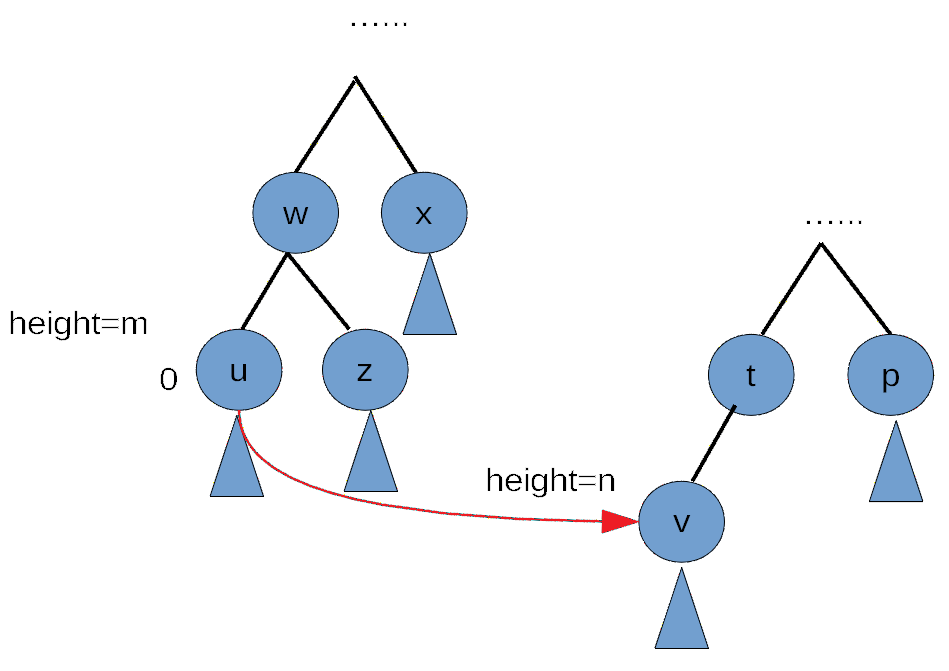
\includegraphics[width=0.5\linewidth]{nondir_case4}
	\caption{Non-Directional Algorithm case 3}
	\label{fig:nondircase4}
\end{figure}

	In this case, let$p$ be the nearest common parent of $u$ and $v$ and $w$ and $x$ be its child nodes.just as the figure below shows:
	\begin{figure}[H]
		\centering
		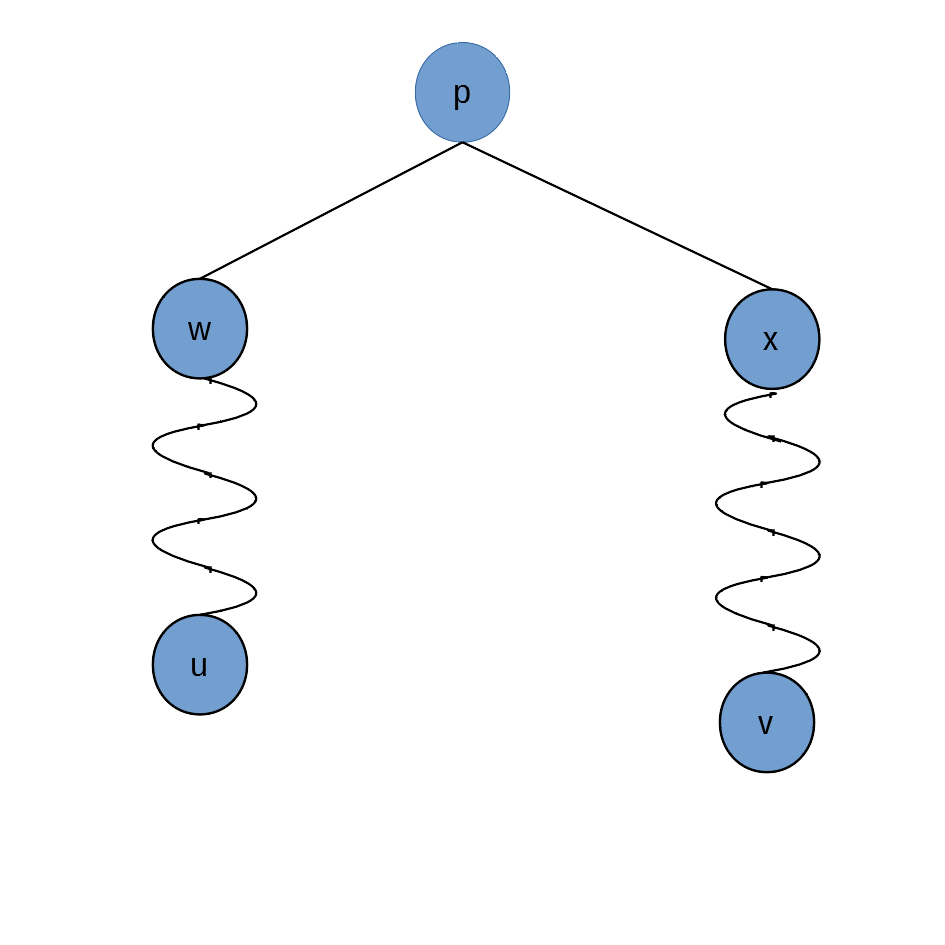
\includegraphics[width=0.5\linewidth]{nondir_case3def}
		\caption{Non-Directional Algorithm case 3 transform }
		\label{fig:nondircase3def}
	\end{figure}
	Similar to case 2's proof, we will prove this by induction. Assuming that directional algorithm is faster than or equal to non-directional algorithm for trees of height 1,2,...,n-1. For nor-tree of height n, Here are several small cases here:
	\begin{enumerate}
		\item The non-directional algorithm continue visit the sub tree containing $v$;
		\item The  non-directional algorithm jump back to $u$ to visit that sub tree.
		\item The non-directional algorithm jump to different subtrees randomly.
	\end{enumerate}
	
	\begin{proof}
		Let $P,X,W$ be situation when $w=0,x=0$, $w=0,x=1$ and $w=1,x=0$.et $E(c(s))$ be the expected cost of an vertex $s$ in directional algorithm and $E(c_N(s))$ be the expected cost of an vertex $s$ in non-directional algorithm.
		
		The expected cost of directional algorithm is:
		\begin{equation}
		\begin{split}
		    E(c(p))=Pr[P]E[c(w)|P]+Pr[P]E[c(x)|P]+Pr[X]E[c(w)|X] \\
		        +Pr[X]E[c(x)|X]+Pr[W]E[c(w)|W]
		\end{split}
		\end{equation}
		
		For non-directional algorithm continue visit the sub tree containing $v$:
		\begin{equation}
		\begin{split}
		   E(c_N(p))=Pr[P]E[c_N(w)|P]+Pr[P]E[c_N(x)|P]+Pr[X]E[c_N(u)|X] \\
		   +Pr[X]E[c_N(x)|X]+Pr[W]E[c_N(w)|W]+Pr[W]E[c_N(x)|W]
		\end{split}
		\end{equation}
		
		For non-directional algorithm jump back to $u$ to visit that sub tree:
		\begin{equation}
		\begin{split}
		E(c_N(p))=Pr[P]E[c_N(w)|P]+Pr[P]E[c_N(x)|P]+Pr[X]E[c_N(w)|X]\\
		+Pr[X]E[c_N(x)|X]+Pr[W]E[c_N(w)|W]+Pr[W]E[c_N(v)|W]
		\end{split}
		\end{equation}
		
		For the algorithm continue visit the sub tree containing $v$:
		\begin{equation}
		E(c_N(p))-E(c(p))\ge Pr[W]E[c_N(x)|W]-Pr[X]E[c(w)|X]+Pr[X]E[c_N(u)|X]
		\end{equation}
		
		Based on the assumption: $E[c_N(x)|W]=E[c_N(w)|X]$, the algorithm jump back to $u$ to visit that sub tree:
		$$E(c_N(p))-E(c(p))\ge Pr[W]E[c_N(v)|W]$$
		
		Therefore we could conclude that directional algorithm is faster than the non-directional one in this case.
	\end{proof}
	
	
	
	